% Reconstruction in LArTPC
% Target length: 30 pages

\graphicspath{{LArTPCReconstruction/Figs/}}

%----------------------------------------------------------------------------------------------------------------------------------------------------------------------------
\chapter{Reconstruction in a Liquid Argon TPC}\label{chap:LArTPCReconstruction}

{\color{red} Should the title of this chapter reflect more of the original work which is discussed within?  e.g. Shower Reconstrucion in a Liquid Argon TPC?  Although  it is a general reconstruction chapter, everything in Shower Reconstruction in LArTPCs is original.}

The use of LArTPCs in future high-precision projects, such as long-baseline neutrino experiments, is very well motivated by the unprecedented spatial and energy resolution available to detectors utilising the techonology.  In order to take advantage of all this accessible information, accurate reconstruction must be developed to perform pattern recognition and energy determination for use by the proceeding analyses.  The techniques and status of reconstruction in LArTPCs is the subject of this chapter, with particular focus on novel methods developed for the reconstruction of electromagnetic showers.

The implementation of the reconstruction algorithms discussed in this chapter utilises the Liquid Argon Software framework (LArSoft), developed at FNAL and shared between all experiments in the LAr program.  LArSoft will be overviewed in Section~\ref{sec:LArSoft} before the structural and calorimetric reconstructions are discussed in Sections~\ref{sec:ReconstructionChain} and~\ref{sec:Calorimetry} respectively.  The development of new techniques in the reconstruction of showers will compose the main discussion in this chapter and is contained in Section~\ref{sec:ShowerReconstruction}.

%----------------------------------------------------------------------------------------------------------------------------------------------------------------------------
\section{The LArSoft Framework}\label{sec:LArSoft}

The Liquid Argon Software (LArSoft) \cite{LArSoftWebsite,LArSoft2013,LArSoft2016,Snider2016} collaboration supports the development, use, sharing and distributing of code utlitised by all LAr experiments at FNAL.  The LArSoft framework is written in C++ and built on \textit{art} \cite{artWebsite,art2012}, the event-processing system develop at FNAL and used by offline code developed for most experiments hosted at the lab.  As data from most LArTPC experiments share a similar basic format, LArSoft is envisioned to be agnostic to the detector specifics and provide a common interface, infrastructure and algorithms for simulation, reconstruction and analysis.  Along with vastly reducing duplicated effort, this also allows access to the most advanced software developments for smaller collaborations who otherwise may not have the required resources.

LArSoft provides well defined interfaces to various external packages, such as GENIE \cite{GENIE2010} and GEANT4 \cite{GEANT42006}, and access by particular experiments utilises configurable descriptions of the detector geometry, the electronics, detector response and other unique features.  This structure is demonstrated in Figure~\ref{fig:LArSoftStructure}.  This architecture ensures a flexible structure which facilitates the addition and evolution of algorithms and with contigency for future developments to be introduced with ease.

\begin{figure}
  \centering
  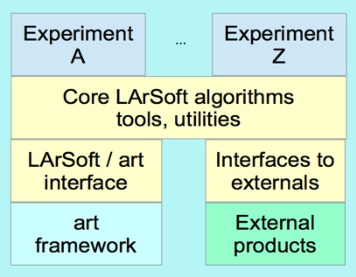
\includegraphics[width=7cm]{LArSoftStructure.pdf}
  \caption[The LArSoft architecture, highlighting support for both common and experiment-specific algorithms and methods and the interfacing with other packages.]{The LArSoft architecture, highlighting support for both common and experiment-specific algorithms and methods and the interfacing with other packages.  Taken from \cite{LArSoft2016}.}
  \label{fig:LArSoftStructure}
\end{figure}

The \textit{art} framework provides an interface to the information stored for each event by user-written `modules' and handles execution by processing each entry and making the data available to these plug-in modules.  Additionally, `services', which exist outside of the event structure, are provided and may be used to obtain general information such as detector geometry or LAr properties whenever needed.  The two main module types, named \texttt{Analyzers} (sic) and \texttt{Producers}, can access the data products stored in a particular event and, in the case of \texttt{Producers}, have the ability to place data into the event for use in future processes.  All modules, regardless of their type, have only \texttt{const} access to the existing information in the event.  Configuration of an \textit{art} job utilises the custom Fermilab Hierarchical Configuration Language (\textit{fhicl}, pronounced `fickle') which may be used to define the modules (including their order) and services to be run and to provide run-time parameters for use by these products.

The end-to-end configuration for a given experiment involves the following standard stages: generation (provided by a generator, such as GENIE), propagation (executed with GEANT4), detector response simulation, and reconstruction.  The results from the first three steps aim to reproduce as closely as possible the expectations from real data, with the same reconstruction applied to both the simulated output from the detector and data.  The processes are configured, using \texttt{Producer} modules, in \textit{art} using \textit{fhicl}, generally separated into four jobs representing each of the stages.

LArSoft was initially developed for use in ArgoNeuT in around 2011 and has since progressed into the large collaboration which it is today, with more than 100 code authors spanning multiple experiments.  The constant progression of algorithms have resulted in very well-developed, advanced simulation and reconstruction tools with corresponding shared expertise.  The recent uses of LArSoft reconstruction on real data, in MicroBooNE \cite{MicroBooNEReconstruction2017} and the 35~ton (Chapter~\ref{chap:35tonAnalysis}), are providing an excellent test of the efficacy of the simulation along with the validation of reconstruction applied to data.  The current reconstruction chain is discussed in Section~\ref{sec:ReconstructionChain} and the process of calorimetry in a LArTPC and the LArSoft implementation is the subject of Section~\ref{sec:Calorimetry}.

Until recently, convincing electromagnetic shower reconstruction has not existed within LArSoft.  Despite this being a major advantage of LArTPCs, it is particularly challenging and requires significant investment of resources to fully understand.  This motivated the development of new algorithms within the LArSoft framework, BlurredCluster and EMShower, which will be discussed in detail in Section~\ref{sec:ShowerReconstruction}.

%----------------------------------------------------------------------------------------------------------------------------------------------------------------------------
\section{The Reconstruction Chain}\label{sec:ReconstructionChain}

Reconstruction in LArSoft is the process of forming particle objects, with enough information to be able to perform identification, from the raw charge read out by the anode planes.  The process may be considered as three main components: calibrating the raw charge to remove detector effects; pattern recognition; calorimetry.  The general workflow is shown schematically in Figure~\ref{fig:ReconstructionWorkflow}.

\begin{figure}
  \centering
  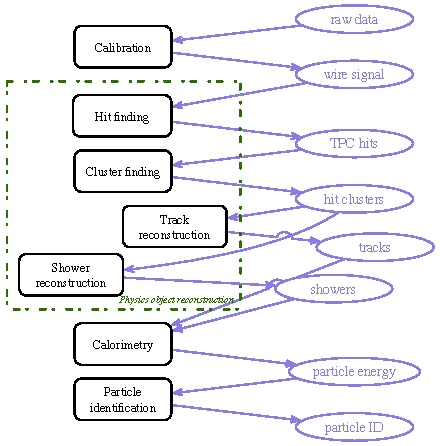
\includegraphics[width=8cm]{ReconstructionWorkflow.pdf}
  \caption[The LArSoft reconstruction workflow to produce 3D reconstructed objects from the raw charge read out by the anode wires.]{The LArSoft reconstruction workflow to produce 3D reconstructed objects from the raw charge read out by the anode wires \cite{LArSoft2016}.  The status of the reconstruction is shown on the right, with the various algorithms and their outputs represented on the left.}
  \label{fig:ReconstructionWorkflow}
\end{figure}

%----------------------------------------------------------------------------------------------------------------------------------------------------------------------------
\subsection{From Charge to Hits}\label{sec:HitReconstruction}

The charge induced and collected on the readout wires is modified by detector effects which must be well understood in order to be properly accounted for.  The measured waveform, $p(t)$, obtained from the signal $s(t)$, measured as a function of time $t$, can be represented in pseudocode as
\begin{equation}
  p(t) = \left( s(t) \otimes e(t) \otimes f(t) \right) + n(t),
\end{equation}
where $e$ is the electronics response, $f$ is the field response and $n$ is the noise in the detector.  Together, $e(t) \otimes f(t)$ are referred to as the detector response.

The first step in the reconstruction, referred to as the `deconvolution stage', involves removing these detector responses.  This proceeds by subtracting the noise profile from the measured waveform before Fourier transforming into frequency space and dividing out the field and electronics components.  The detector responses must be accurate and the models used have been developed at test stands to ensure they best represent the detector effects.  This process is applied in reverse during the detector simulation stage of the simulation to reproduce the expectations from the data as much as possible.

Following the deconvolution stage, the waveforms all have the form of a unipolar pulse.  The reconstruction proceeds with `hit finding', with the purpose to accurately determine the properties of the collected charge.  In particular, the peak time, width and total charge of the `hit's are pertinent for future reconstruction algorithms.  This is typically achieved by fitting a Gaussian to the pulse and using this to aid the determination of the hit properties.  The result of the deconvolution and hit finding stages are represented for simulated hits on three separate planes in Figure~\ref{fig:HitFinding}.

\begin{figure}
  \centering
  \begin{subfigure}[t]{0.3\linewidth}
    \centering
    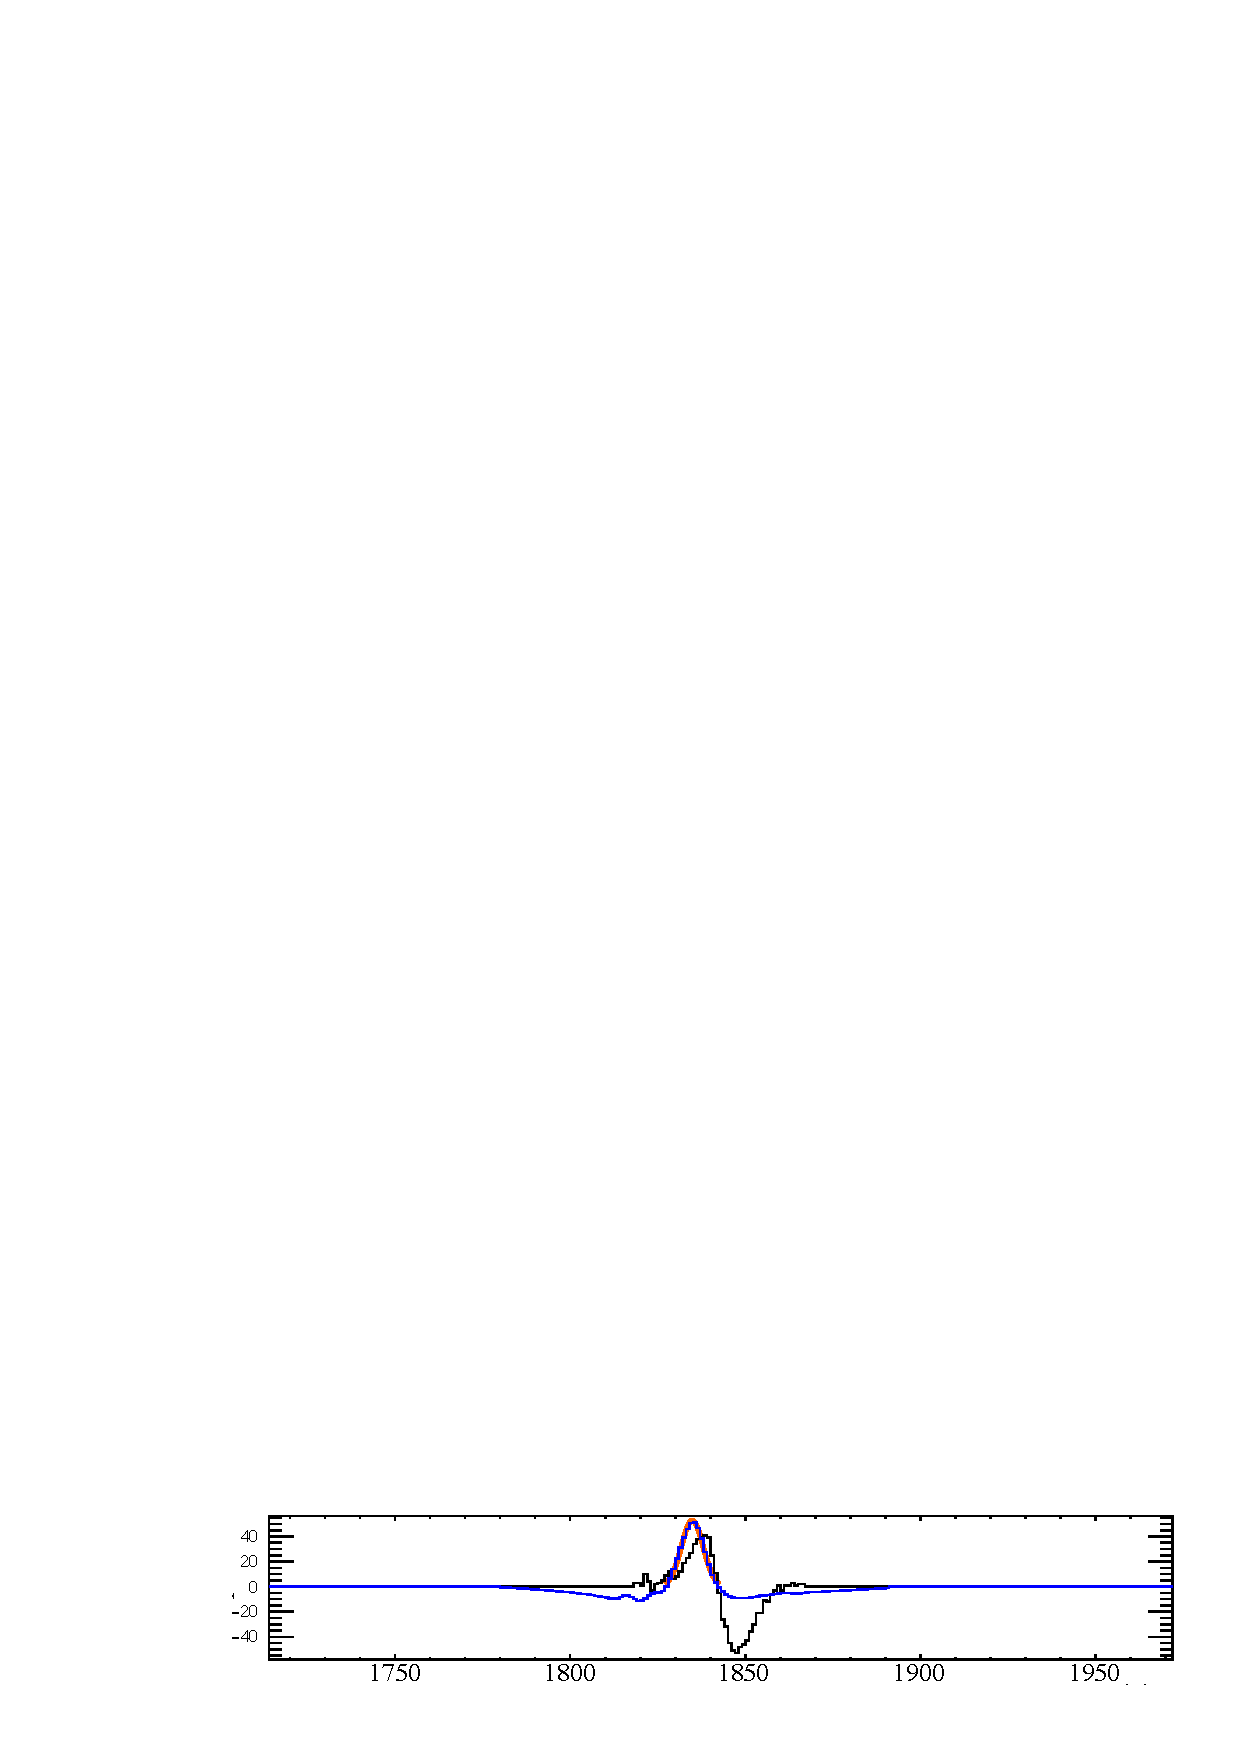
\includegraphics[width=\textwidth]{HitFindingU.pdf}
    \caption{U plane.}
    \label{fig:HitFindingU}
  \end{subfigure}
  \hfill
  \begin{subfigure}[t]{0.3\linewidth}
    \centering
    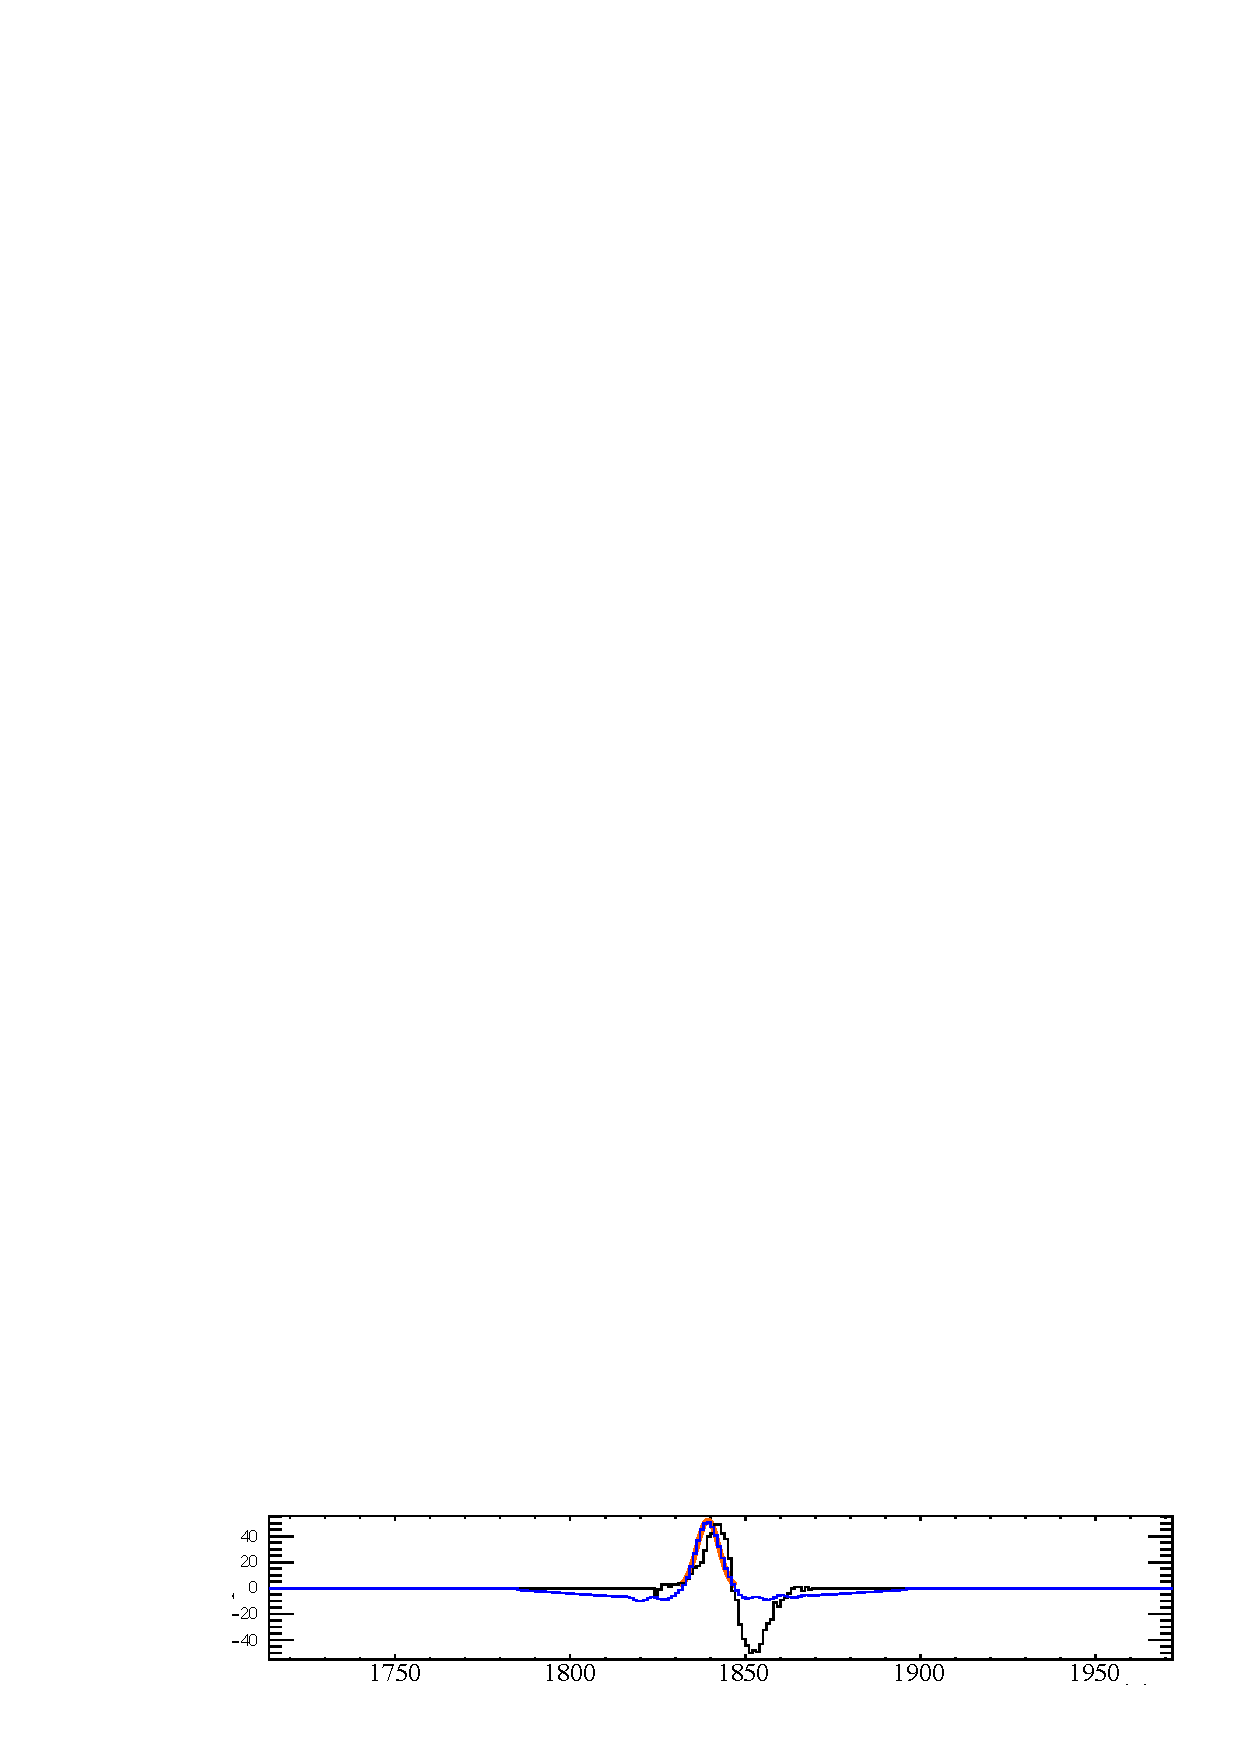
\includegraphics[width=\textwidth]{HitFindingV.pdf}
    \caption{V plane.}
    \label{fig:HitFindingV}
  \end{subfigure}
  \hfill
  \begin{subfigure}[t]{0.3\linewidth}
    \centering
    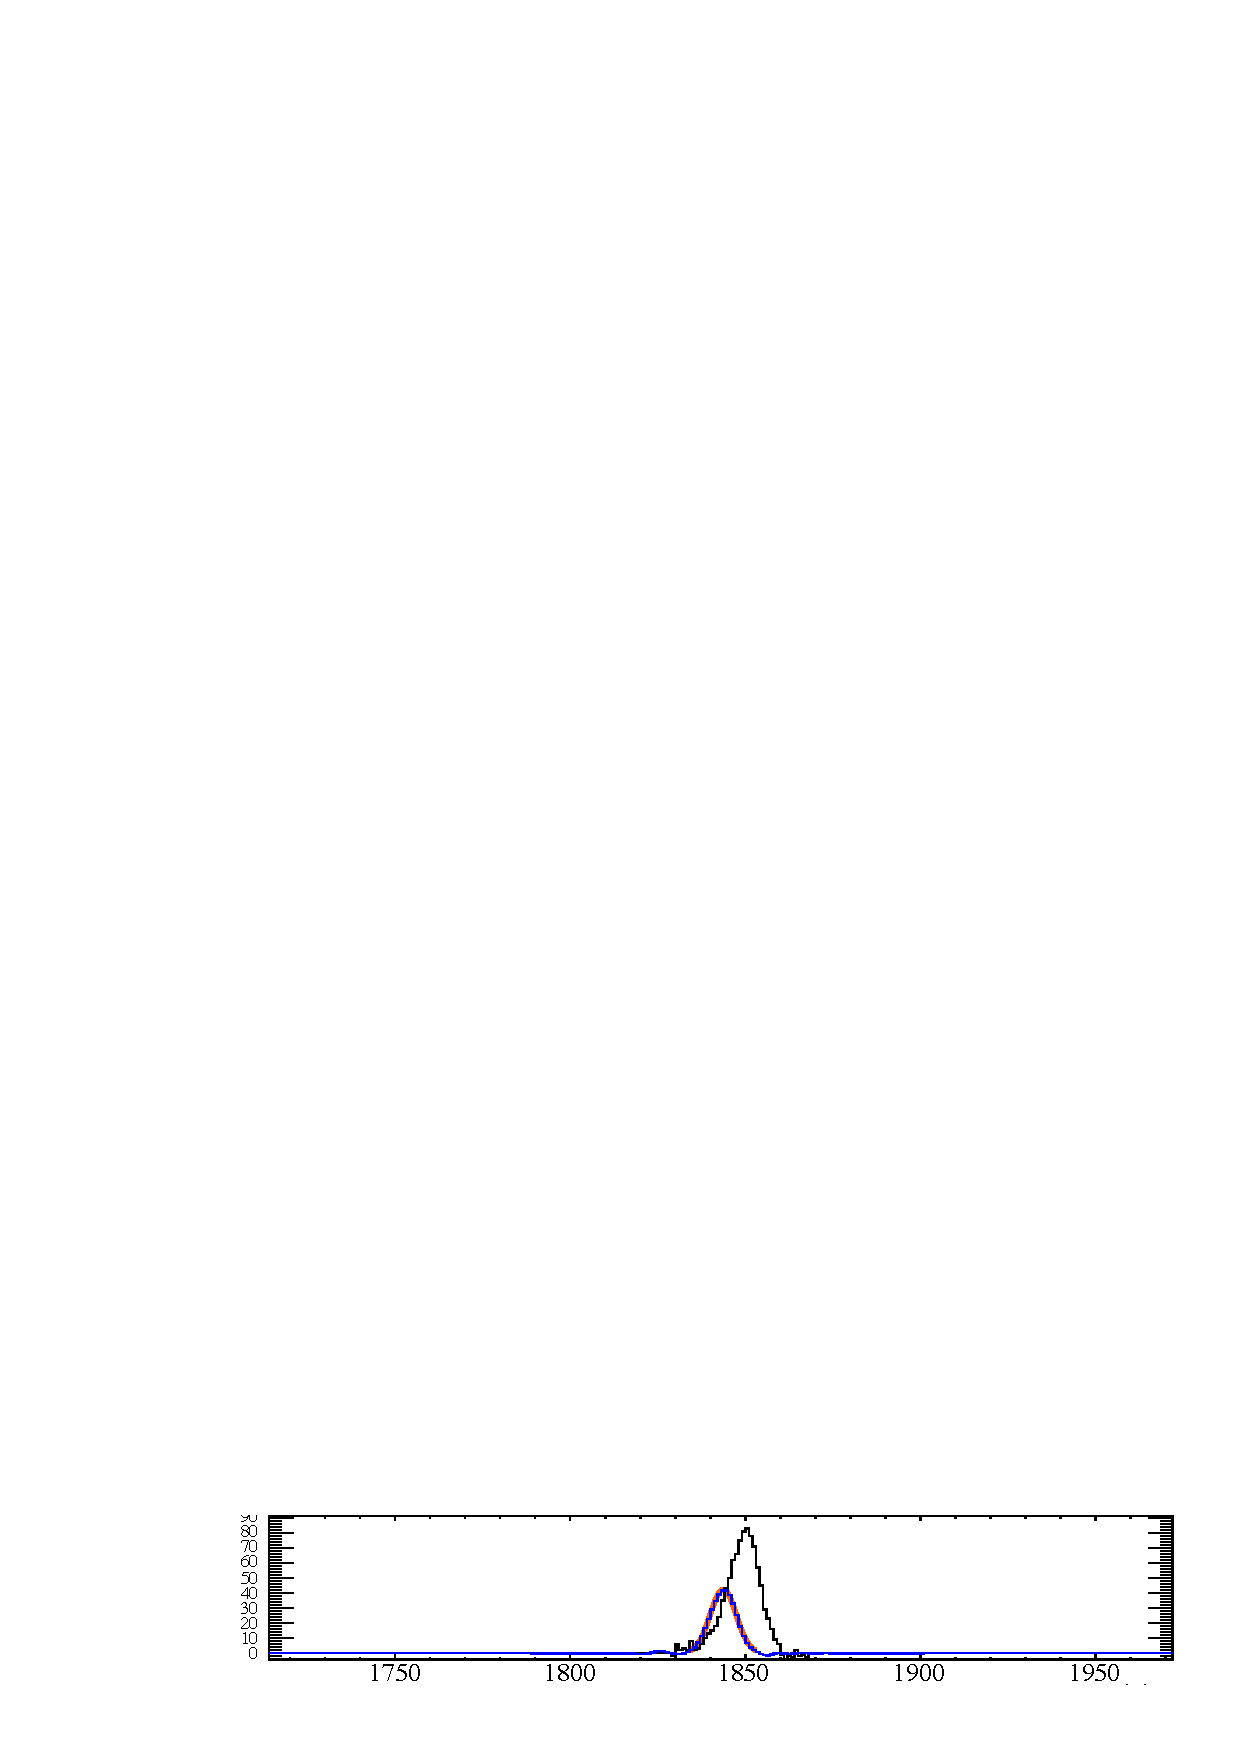
\includegraphics[width=\textwidth]{HitFindingZ.pdf}
    \caption{Z plane.}
    \label{fig:HitFindingZ}
  \end{subfigure}
  \caption[The process of deconvolution and hit finding to determine the correct charge from the measured pulses on the readout wires.]{The process of deconvolution and hit finding to determine the correct charge from the measured pulses on the readout wires.  Each 2D plane is represented as charge (ADC) as a function of time (tick).  In each case, the black waveform represents the raw measurement, the blue shows the outcome of deconvolution and the pink peak indicates the reconstructed hit.  Note the normalisation of the deconvoluted signal has been fixed to provide a factor four amplification for illustratory purposes.  The shift in time and shape is a result of the deconvolution from the electronics response (demonstrated in Figure~\ref{fig:ElectronicsResponse}).}
  \label{fig:HitFinding}
\end{figure}

Due to the wrapped wires, multiple hits will be reconstructed on each channel, one for each possible wire segment.  The final stage of hit processing is to perform disambiguation to select the correct hit for use in subsequent algorithms.  As previously discussed (Section~\ref{sec:DUNESinglePhase} and Section~\ref{sec:35tonTPC}), this is trivial in the far detector design as the wire wrapping angles are chosen such that no induction wire segment crosses each collection channel more than once.  In the 35~ton, the slight difference in angle between the two induction planes results in `triple points', where there are hits on each plane almost instantaously, which facilitates a deduction of the correct induction channel hits.

%----------------------------------------------------------------------------------------------------------------------------------------------------------------------------
\subsection{Object Reconstruction}\label{sec:ObjectReconstruction}

The next typical stage of the reconstruction following hit finding is the process of forming 2D objects, or `clustering'.  In LArSoft, all 2D objects, regardless of their topology, are named `clusters' and are simply a collection of hits identified as being associated with a common ionising particle.  These 2D structures exist only on a given plane and do not have contributions from multiple views; the extension to 3D reconstruction involves combining numerous clusters between the views.  Multiple cluster algorithms exist in LArSoft, each designed for different specialisations.

An example 2D view of a $\nu_{\mu}$CC event, simulated in a reduced far detector volume, is shown in Figure~\ref{fig:2DnumuCC}.  This particular interaction is $nu$.  The outcome of hit reconstruction is demonstrated in Figure~\ref{fig:2DnumuCCHits} and the result of applying clustering to these hits is displayed in Figure~\ref{fig:2DnumuCCClusters}, with each colour representing a separate cluster.

\begin{figure}
  \centering
  \begin{subfigure}[t]{0.48\linewidth}
    \centering
    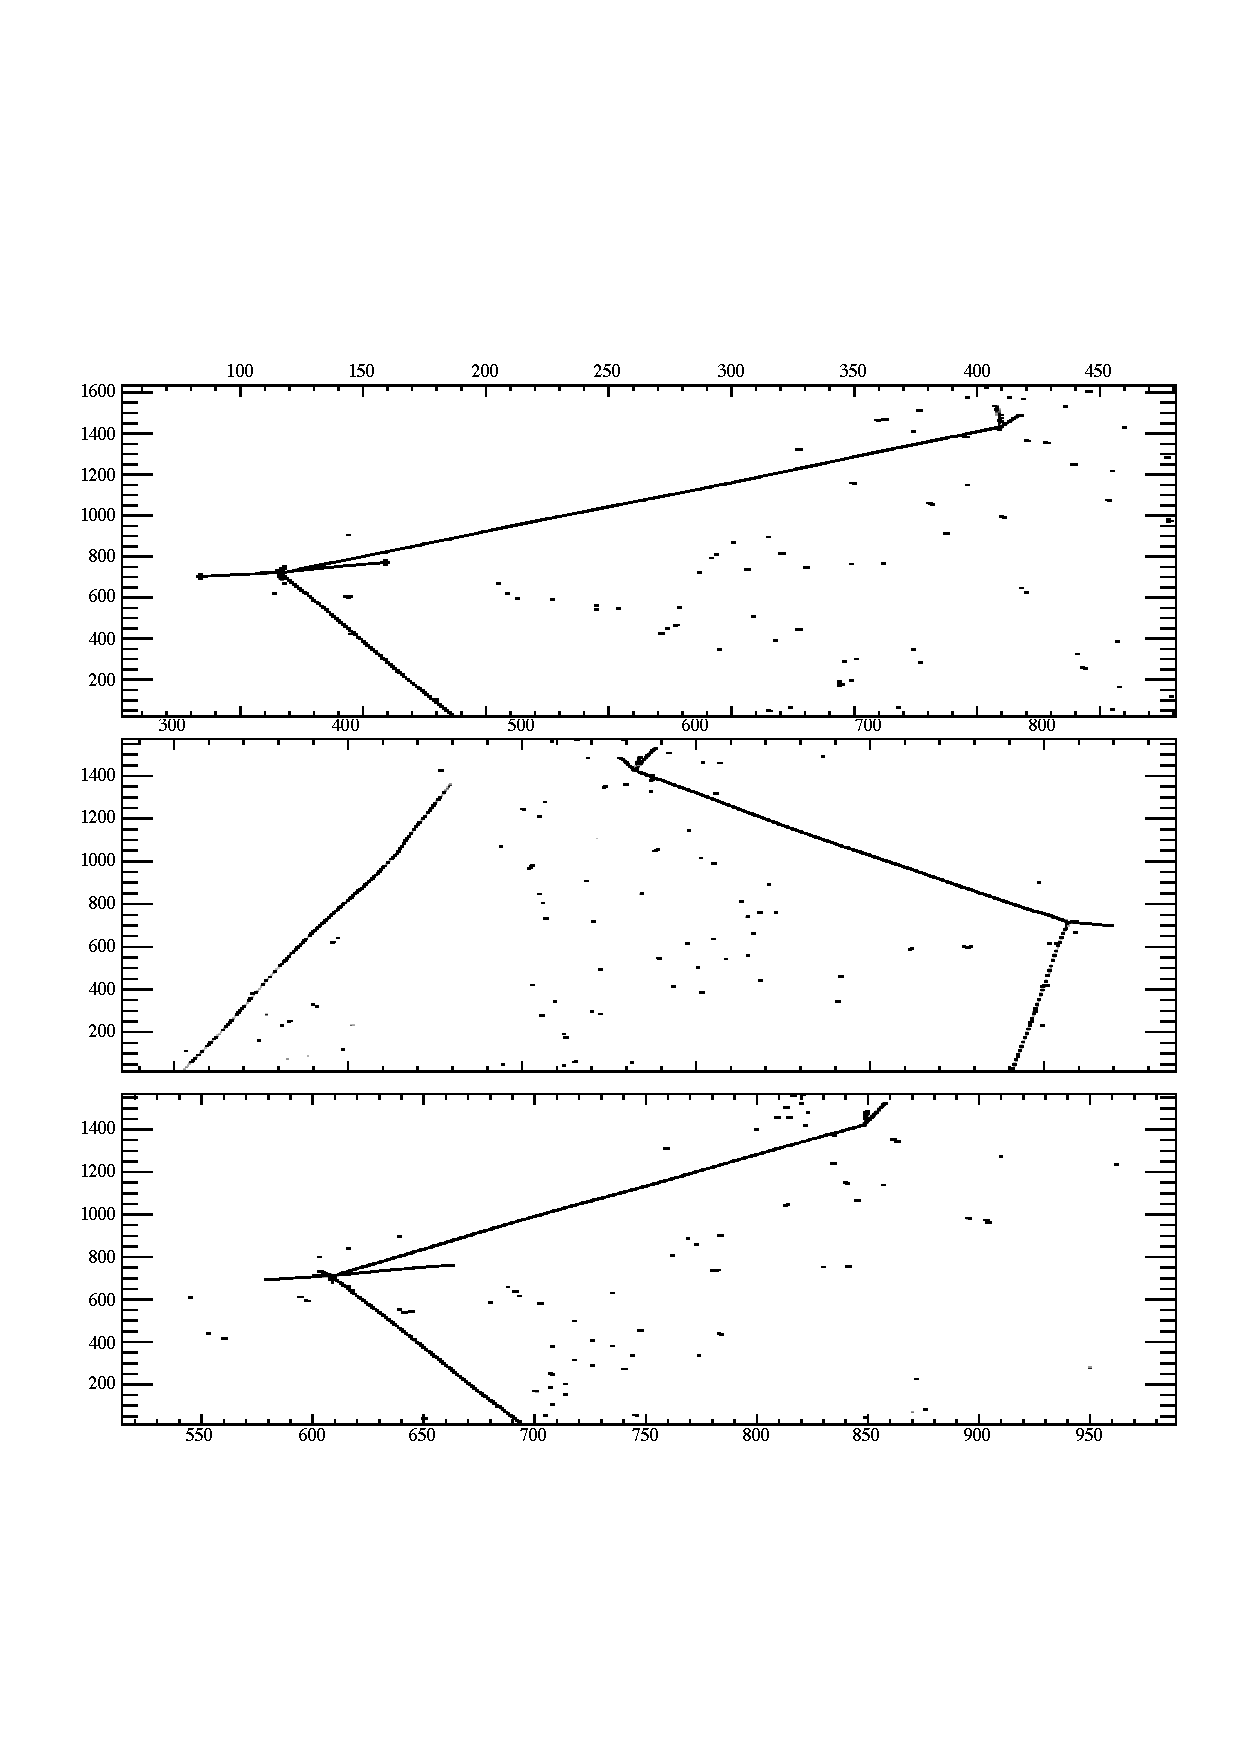
\includegraphics[width=0.98\textwidth]{2DnumuCCHits.pdf}
    \caption{Hit reconstruction.}
    \label{fig:2DnumuCCHits}
  \end{subfigure}
  \hfill
  \begin{subfigure}[t]{0.48\linewidth}
    \centering
    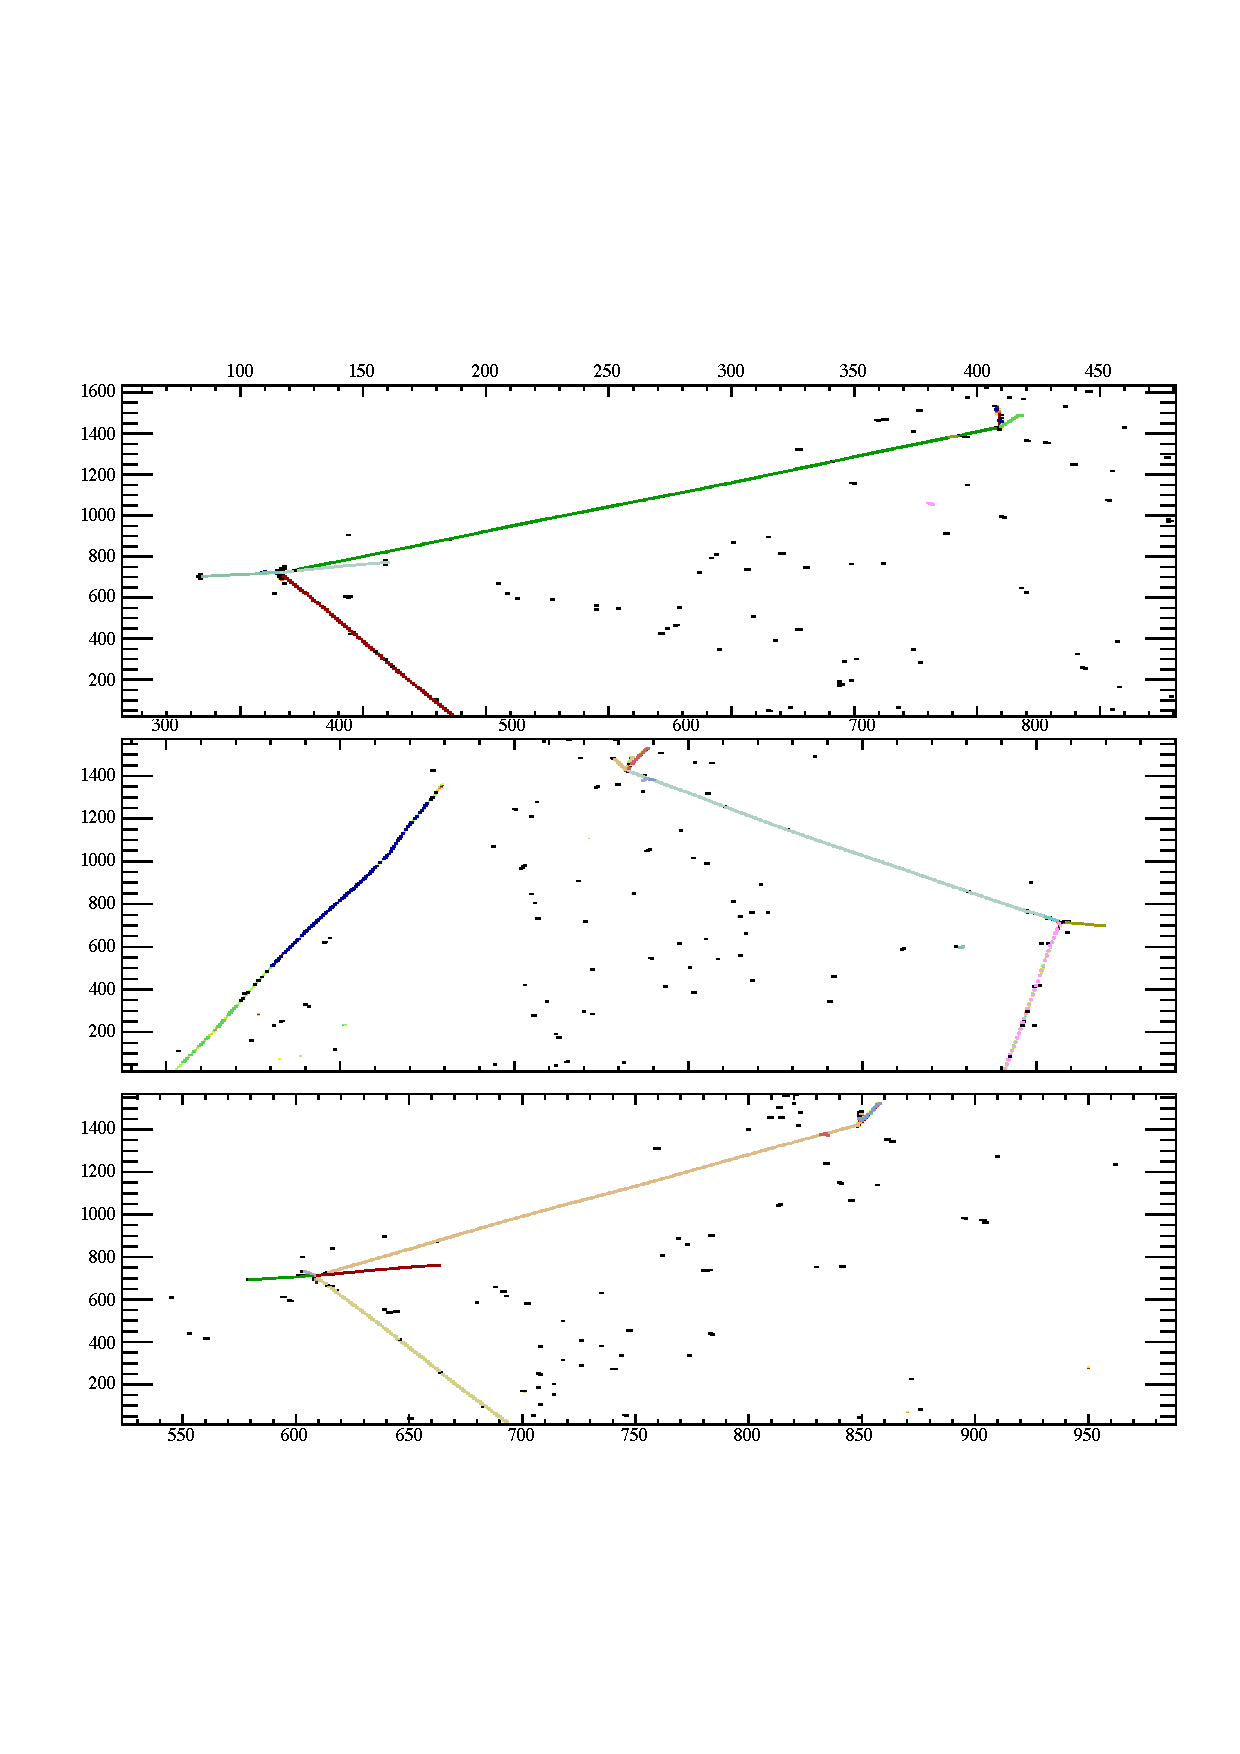
\includegraphics[width=0.98\textwidth]{2DnumuCCClusters.pdf}
    \caption{Cluster reconstruction.}
    \label{fig:2DnumuCCClusters}
  \end{subfigure}
  \caption{}
  \label{fig:2DnumuCC}
\end{figure}

Combining 2D information from multiple views in a LArTPC enables the formation of 3D objects.  In LArSoft, several 3D products exist: `space points', `vertices', `tracks' and `showers'.  Space points are a form of 3D hit and are defined by a point in the detector Cartesian geometry and vertices are a specific example of these locations, created to represent an important part of the event (e.g. the neutrino interation point or even just the start of a track).  Tracks and showers are more complete objects which represent individual particles and contain associated properties relevant to the topology of each.  Tracking is relatively advanced in LArSoft, with multiple track fitters shown to produce well-formed track objects efficiently; shower reconstruction is less so and will be discussed in detail in Section~\ref{sec:ShowerReconstruction}.

The result of applying track reconstruction to the $\nu_{\mu}$CC interaction discussed in Figure~\ref{fig:2DnumuCC} is shown in Figure~\ref{fig:3DnumuCC}.  As with clusters, each colour represents a unique track object and it is clear from Figure~\ref{fig:3DnumuCC2D} that hits across multiple planes contribute to a given track.  A separate view is also shown in Figure~\ref{fig:3DnumuCC3D}, where the objects are represented in two orthogonal views in the detector coordinate system.

\begin{figure}
  \centering
  \begin{subfigure}[t]{0.48\linewidth}
    \centering
    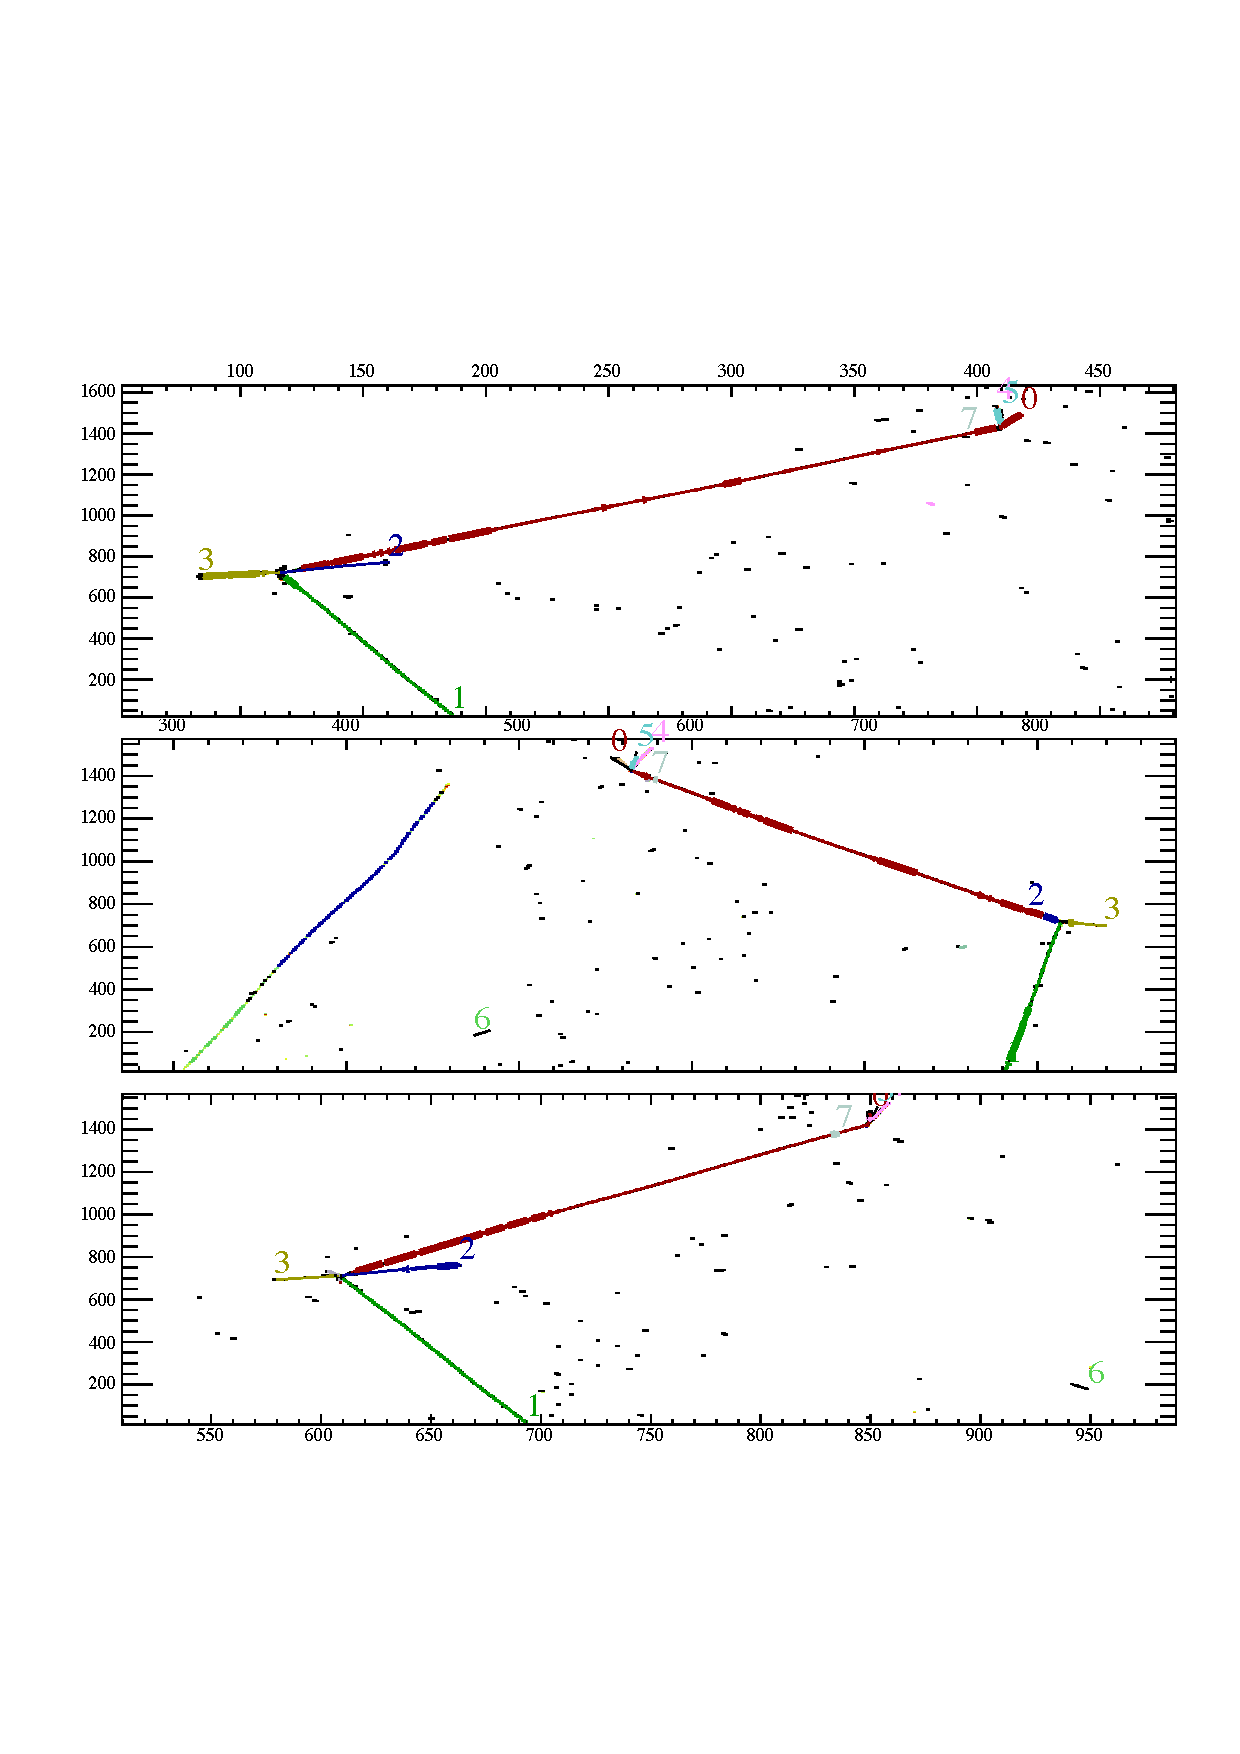
\includegraphics[width=0.98\textwidth]{3DnumuCC2D.pdf}
    \caption{2D view; wire vs tick for multiple wire planes.}
    \label{fig:3DnumuCC2D}
  \end{subfigure}
  \hfill
  \begin{subfigure}[t]{0.48\linewidth}
    \centering
    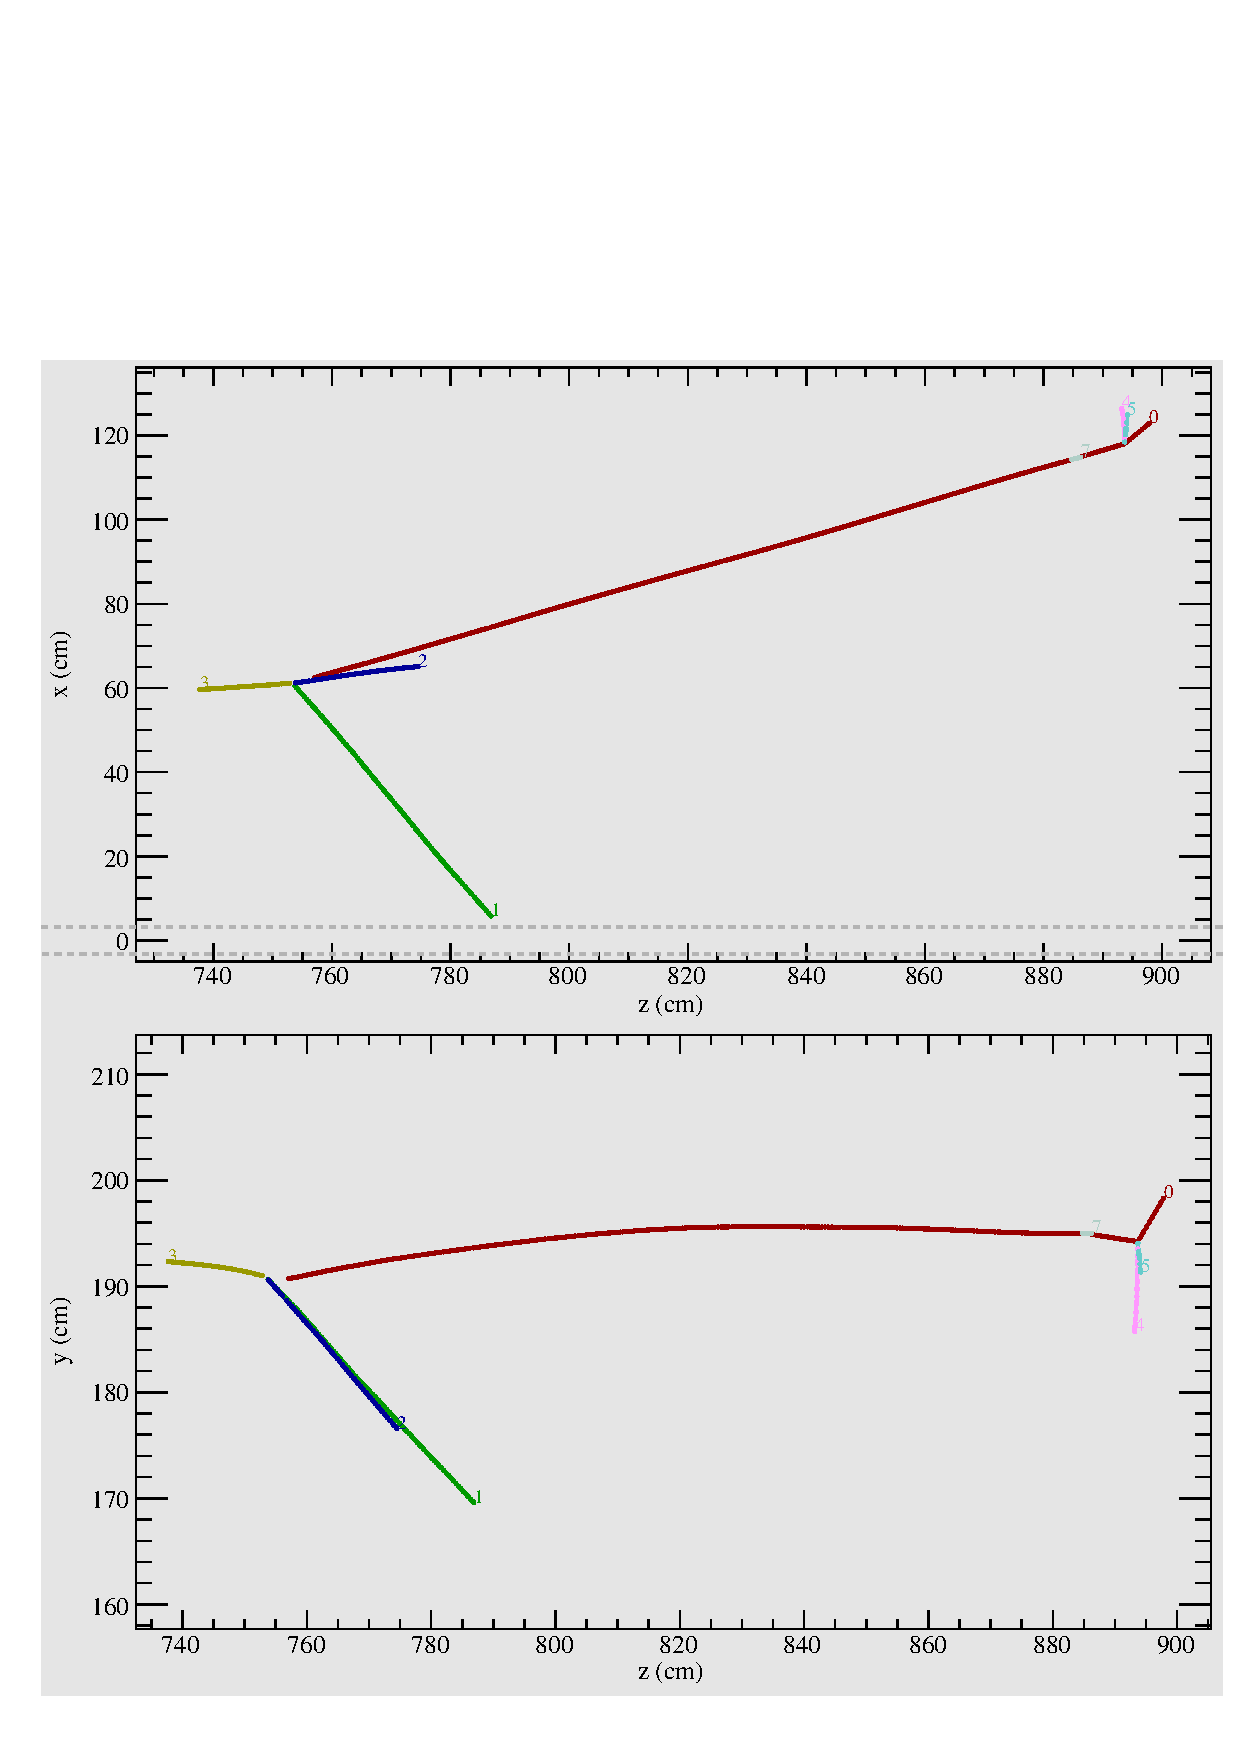
\includegraphics[width=0.98\textwidth]{3DnumuCC3D.pdf}
    \caption{3D view; $x$-$z$ and $y$-$z$ othogonal planes.}
    \label{fig:3DnumuCC3D}
  \end{subfigure}
  \caption{}
  \label{fig:3DnumuCC}
\end{figure}

It is worth noting the approach to forming the eventual 3D objects, from which particle identification and analysis may be executed, is not unique.  The method outlined above is most relevent to the shower reconstruction discussed in Section~\ref{sec:ShowerReconstruction} and is the most common chain used in most LArSoft processing; however, progress is being made on an additional technique which focusses directly on 3D reconstruction.  This is called `Wire-Cell' \cite{WireCellWebsite} and utilises a tomographic method, following the LArTPC principal that each plane observes the same amount of ionisation electrons, to build up a 3D image of the event.  This may then be characterised to find the properties of the particles and make the track and shower products.  All reconstruction methods utilise the same information provided by the detector but not necessarily in the same order.

%----------------------------------------------------------------------------------------------------------------------------------------------------------------------------
\subsection{Calorimetry Reconstruction}\label{sec:Calorimetry}

The extremely precise energy measurements is a hugely attractive features of LArTPCs and is achieved by careful calibration of the charge recieved from the drift electrons.  Following deconvolution and hit finding, the charge carried by each packet of electrons is understood as the Gaussian integral of the hit and has units 10~e$^-$ (often just `ADC' in certain following plots).  This is converted to an energy

%----------------------------------------------------------------------------------------------------------------------------------------------------------------------------
\section{Shower Reconstruction in LArTPCs}\label{sec:ShowerReconstruction}

%----------------------------------------------------------------------------------------------------------------------------------------------------------------------------
\subsection{Showers Overview}\label{sec:ShowersOverview}

%----------------------------------------------------------------------------------------------------------------------------------------------------------------------------
\subsection{BlurredCluster Algorithm}\label{sec:BlurredCluster}

%----------------------------------------------------------------------------------------------------------------------------------------------------------------------------
\subsection{EMShower Algorithm}\label{sec:EMShower}

%----------------------------------------------------------------------------------------------------------------------------------------------------------------------------
\subsection{Track/Shower Separation}\label{sec:TrackShowerSeparation}

%----------------------------------------------------------------------------------------------------------------------------------------------------------------------------
\subsection{Performance of the Reconstruction}\label{sec:ReconstructionPerformance}
